\documentclass{article}
\usepackage{amsmath}
\usepackage{tikz}
\usetikzlibrary{matrix}

\begin{document}

\begin{figure}[h]
    \centering
    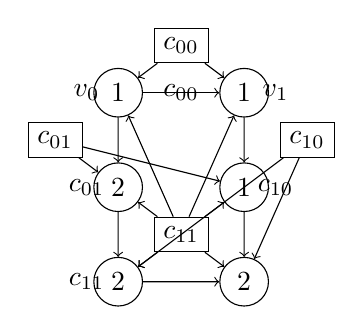
\begin{tikzpicture}[scale=0.8]
        % Define nodes for the cubes
        \node (c00) [draw, rectangle] at (0,0) {$c_{00}$};
        \node (c01) [draw, rectangle] at (-2,-1.5) {$c_{01}$};
        \node (c10) [draw, rectangle] at (2,-1.5) {$c_{10}$};
        \node (c11) [draw, rectangle] at (0,-3) {$c_{11}$};

        % Define nodes for the vertices
        \node (v0) [circle, draw, fill=white] at (-1,-0.75) {1};
        \node (v1) [circle, draw, fill=white] at (1,-0.75) {1};
        \node (v2) [circle, draw, fill=white] at (-1,-2.25) {2};
        \node (v3) [circle, draw, fill=white] at (1,-2.25) {1};
        \node (v4) [circle, draw, fill=white] at (-1,-3.75) {2};
        \node (v5) [circle, draw, fill=white] at (1,-3.75) {2};

        % Draw edges between the vertices
        \draw[->] (v0) -- (v1);
        \draw[->] (v0) -- (v2);
        \draw[->] (v1) -- (v3);
        \draw[->] (v2) -- (v4);
        \draw[->] (v3) -- (v5);
        \draw[->] (v4) -- (v5);

        % Draw edges between the cubes
        \draw[->] (c00) -- (v0);
        \draw[->] (c00) -- (v1);
        \draw[->] (c01) -- (v2);
        \draw[->] (c01) -- (v3);
        \draw[->] (c10) -- (v4);
        \draw[->] (c10) -- (v5);
        \draw[->] (c11) -- (v0);
        \draw[->] (c11) -- (v1);
        \draw[->] (c11) -- (v2);
        \draw[->] (c11) -- (v3);
        \draw[->] (c11) -- (v4);
        \draw[->] (c11) -- (v5);

        % Add labels for the vertices
        \node at (-1.5, -0.75) {$v_0$};
        \node at (1.5, -0.75) {$v_1$};
        \node at (-1.5, -2.25) {$c_{01}$};
        \node at (1.5, -2.25) {$c_{10}$};
        \node at (-1.5, -3.75) {$c_{11}$};
        \node at (0, -0.75) {$c_{00}$};
    \end{tikzpicture}
    \caption{A 2-cube induced in $\mathcal C_3(P_3)$ by generator $(\set{v_0,v_1},\set{c_{00},c_{01},c_{10},c_{11}})$ with colors $k_{0,0}=1, k_{0,1}=2, k_{1,0}=1,k_{1,1}=2$, using the notation of Lemma~\ref{lem:cubeconstruction}.}
    \label{fig:2-cube}
\end{figure}

\end{document}